\documentclass{article}
\usepackage{../../Self_Style}

\title{Phys 115A HW 1}
\author{Zih-Yu Hsieh}
\date{\today}

\begin{document}
\maketitle

\begin{ques}[Discrete statistics at the Tour de France]\label{q1}
Suppose we’re lucky enough to gather all 61 official winners of the Tour de France in one
room, alive and dead. Four people have won it 5 times apiece, one person has won it 4
times, three people have won it 3 times apiece, twelve people have won it 2 times apiece, and
forty-one people have won it once. If we let $N(j)$ represent the number of winners with $j$
victories in the Tour de France, then $N(5) = 4$, $N(4) = 1$, $N(3) = 3$, $N(2) = 12$, $N(1) = 41$,
and all other $N(j)$ for $j \neq 5, 4, 3, 2, 1$ are zero.

(a) Compute $\langle j^2\rangle$ and $\langle j\rangle^2$.

(b) Determine $\Delta j \equiv j-\langle j\rangle$ for each $j$, and compute the standard deviation using Griffiths
Eq. 1.11 (i.e., $\sigma^2 = \langle (\Delta j)^2\rangle$).

(c) Use your results from (a) and (b) to verify Griffiths Eq. 1.12 (i.e., $\sigma =
\sqrt{\langle j^2\rangle - \langle j\rangle^2}$). %changes
\end{ques}

\begin{proof}

    \hfil

    \begin{itemize}
        \item[(a)] First, consider the total number of winners, we get $N_\textmd{tot} = \sum_{i=1}^5 N(i) = 61$ (in particular, since for $j>5$ we have $N(j)=0$, one can exclude all cases for $j>$). So, the probability for $j=1,2,3,4,5$ is given as $\PP(j) = \frac{N(j)}{N_\textmd{tot}}$. Then, the expectation value of $j$ and $j^2$ is given as follow, respectively:
        \begin{align}
            \left<j\right>=\sum_{i=1}^5 j \cdot \PP(j) = 1\cdot \frac{41}{61}+2\cdot \frac{12}{61}+3\cdot\frac{3}{61}+4\cdot\frac{1}{61}+5\cdot \frac{4}{61}=\frac{98}{61}
        \end{align}
        \begin{align}
            \left<j^2\right> = \sum_{j=1}^{5}j^2\cdot\PP(j) = 1\cdot\frac{41}{61}+4\cdot\frac{12}{61}+9\cdot\frac{3}{61}+16\cdot\frac{1}{61}+25\cdot\frac{4}{61}=\frac{232}{61}
        \end{align}
        So, we get $\left<j^2\right>=\frac{232}{61}$, and $\left<j\right>^2 = \left(\frac{98}{61}\right)^2$.

        \item[(b)] For each $j$, the difference from the expectation value $\left<j\right>$ is given as:
        \begin{align}
            &\Delta 1 = 1-\frac{98}{61}=\frac{-37}{61},\quad \Delta 2=2-\frac{98}{61}=\frac{24}{61},\quad \Delta 3=3-\frac{98}{61}=\frac{85}{61}\\
            &\Delta 4=4-\frac{98}{61}=\frac{146}{61},\quad \Delta 5=5-\frac{98}{61}=\frac{207}{61}
        \end{align}
        So, the variance is given as:
        \begin{align}
            \sigma^2=\left<(\Delta j)^2\right> = \sum_{j=1}^5(\Delta j)^2\cdot \PP(j)=\frac{4548}{3721}
        \end{align}
        Hence, the standard deviation $\sigma=\sqrt{\frac{4548}{3721}}\approx 1.106$.

        \item[(c)] If we consider $\left<j^2\right>-\left<j\right>^2 = \frac{232}{61}-\left(\frac{98}{61}\right)^2 = \frac{4548}{3721}=\sigma^2$ found in part (b), hence $\sigma =\sqrt{\left<j^2\right>-\left<j\right>^2}$ in this case.
    \end{itemize}
\end{proof}

\hfil

\begin{ques}[Fun with gaussians]\label{q2}
We’ll encounter physical situations involving gaussian probability densities repeatedly through-
out the course, so now’s a good time to get comfortable with them. If you’re finding yourself
stuck, please take a look at the accompanying note on gaussian integrals on Gauchospace.

(a) Consider the probability density $\rho(x) = A e^{-\lambda(x-\mu)^2}$, where $A,\mu, \lambda$ are positive, real
constants. Determine $A$ using Griffiths Eq. 1.16 (i.e.,
\[
\int_{-\infty}^\infty \rho(x) \, dx = 1).
\]
Find $\langle x\rangle$, $\langle x^2\rangle$, and $\sigma$. Sketch $\rho(x)$.

(b) Consider now the probability density $\rho(x) = A x e^{-\lambda(x-\mu)^2}$ for positive, real $A,\mu, \lambda$.
Determine $A$, $\langle x\rangle$, $\langle x^2\rangle$, and $\sigma$. Sketch $\rho(x)$. Although it is normalizable, can $\rho(x)$
always be considered a probability density?

(c) Now consider the probability density $\rho(x) = A x^2 e^{-\lambda(x-\mu)^2}$ for positive, real $A,\mu, \lambda$.
Determine $A$, $\langle x\rangle$, $\langle x^2\rangle$, and $\sigma$. Sketch $\rho(x)$.

(d) Shifting back to QM, consider the gaussian wavefunction, $\Psi(x) = A e^{-x^2/b^2}$, find $A$
from the normalization condition (remember how the wavefunction relates to the
probability density). For this wavefunction, calculate $\langle x\rangle$, $\langle x^2\rangle$, and $\sigma_x$, as well as
$\langle p\rangle$, $\langle p^2\rangle$, and $\sigma_p$. Test the uncertainty principle on $\sigma_p$ and $\sigma_x$ for this distribution.
\end{ques}
\begin{proof}

    \hfil

    \begin{itemize}
        \item[(a)] First, $\rho(x)=A e^{-\lambda(x-\mu)^2} = A e^{-(\sqrt{\lambda}(x-\mu))^2}$. Hence, if perform the integration, doing substitution $u=\sqrt{\lambda}(x-\mu)$ and $du = \sqrt{\lambda} dx$, we get:
        \begin{align}
            \int_{-\infty}^{\infty}\rho(x)dx = \int_{-\infty}^{\infty}A e^{-(\sqrt{\lambda}(x-\mu))^2}dx = \frac{A}{\sqrt{\lambda}}\int_{-\infty}^{\infty}e^{-u^2}du = A\sqrt{\frac{\pi}{\lambda}}
        \end{align}
        Hence, for the normalization to happen (or the above integral being $1$), we need $A=\sqrt{\frac{\lambda}{\pi}}$.

        \hfil

        To find $\left<x\right>$ and $\left<x^2\right>$, consider the following integrals (using similar substitutions as above):
        \begin{align}
            \left<x\right> &= \int_{-\infty}^{\infty}x\rho(x)dx = \int_{-\infty}^{\infty}x \cdot Ae^{-(\sqrt{\lambda}(x-\mu))^2}dx\\
            &= \frac{1}{\sqrt{\lambda}}\int_{-\infty}^{\infty}\sqrt{\lambda}(x-\mu)Ae^{-(\sqrt{\lambda}(x-\mu))^2}dx+\mu\int_{-\infty}^{\infty}A e^{-(\sqrt{\lambda}(x-\mu))^2}dx\\
            &= \frac{A}{\lambda}\int_{-\infty}^{\infty}ue^{-u^2}du + \mu = \mu
        \end{align}
        \begin{align}
            \left<x^2\right>&= \int_{-\infty}^{\infty}x^2\rho(x)dx=\int_{-\infty}^{\infty}x^2\cdot Ae^{-(\sqrt{\lambda}(x-\mu))^2}dx\\ 
            &= \frac{1}{\lambda}\int_{-\infty}^{\infty}(\sqrt{\lambda}(x-\mu))^2 Ae^{-(\sqrt{\lambda}(x-\mu))^2}dx + \int_{-\infty}^{\infty}2\mu x Ae^{-(\sqrt{\lambda}(x-\mu))^2}dx-\int_{-\infty}^{\infty}\mu^2 Ae^{-(\sqrt{\lambda}(x-\mu))^2}dx\\
            &= \frac{A}{\lambda\sqrt{\lambda}}\int_{-\infty}^{\infty}u^2 e^{-u^2}du + 2\mu\left<x\right>-\mu^2\cdot \int_{-\infty}^{\infty}\rho(x)dx\\ 
            &= \frac{A}{\lambda^\frac{3}{2}}\left(-\frac{1}{2}ue^{-u^2}\bigg|_{-\infty}^{\infty}+\frac{1}{2}\int_{-\infty}^{\infty}e^{-u^2}du\right) + 2\mu^2-\mu^2 =\sqrt{\frac{\lambda}{\pi}}\cdot\frac{1}{\lambda^\frac{3}{2}}\cdot\frac{\sqrt{\pi}}{2}+\mu^2 = \mu^2+\frac{1}{2\lambda}
        \end{align}
        With these values in mind, we get $\sigma=\sqrt{\left<x^2\right>-\left<x\right>^2}=\sqrt{\mu^2+\frac{1}{2\lambda}-\mu^2} = \frac{1}{\sqrt{2\lambda}}$.

        And, the following is a sketch of $\rho(x)$:

        \begin{figure}[h!]
            \centering
            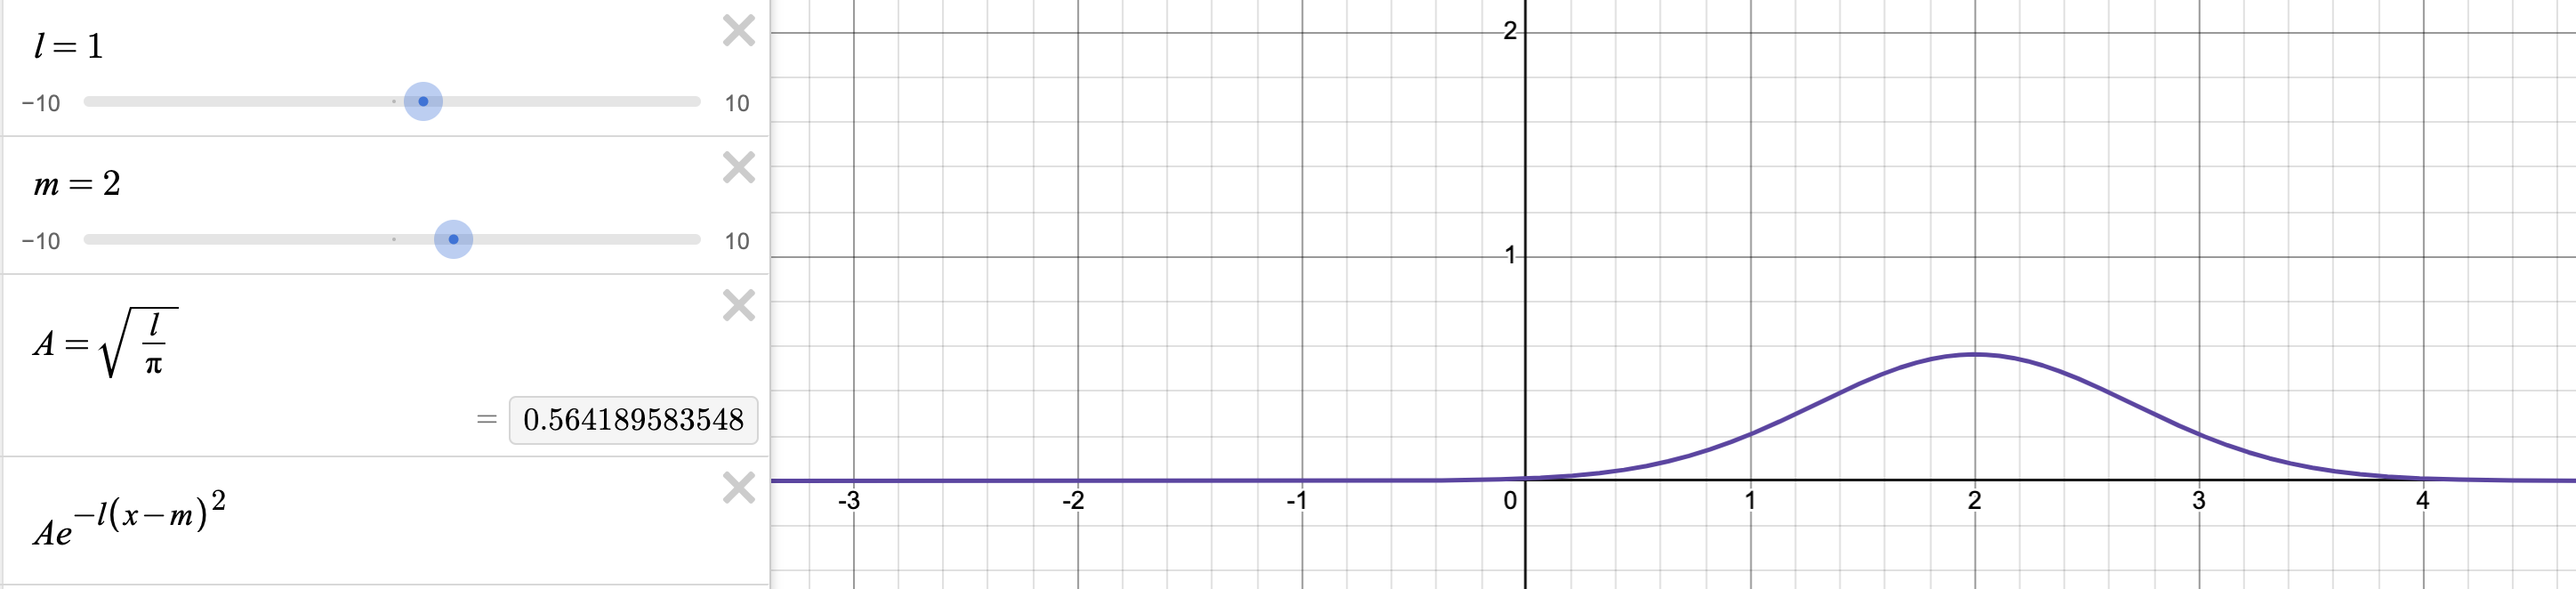
\includegraphics[width=150mm]{q2_a.png}
        \end{figure}

        \hfil

        \item[(b)] If now consider the function $\rho(x)=A xe^{-\lambda(x-\mu)^2}$, where $\rho(x)$ is normalized. To get the constant $A$, consider the following integral (with the same substitution as part (a)):
        \begin{align}
            \int_{-\infty}^{\infty}\rho(x)dx &= \int_{-\infty}^{\infty}A xe^{-(\sqrt{\lambda}(x-\mu))^2}dx = \frac{A}{\sqrt{\lambda}}\int_{-\infty}^{\infty}\sqrt{\lambda}(x-\mu)e^{-(\sqrt{\lambda}(x-\mu))^2}dx + A\mu\int_{-\infty}^{\infty}e^{-(\sqrt{\lambda}(x-\mu))^2}dx\\
            &= \frac{A}{\lambda}\int_{-\infty}^{\infty}ue^{-u^2}du + \frac{A\mu}{\sqrt{\lambda}}\int_{-\infty}^{\infty}e^{-u^2}du = A\mu\sqrt{\frac{\pi}{\lambda}}
        \end{align}
        Hence, for normalization to happen (or the above integral is $1$), we need $A=\sqrt{\frac{\lambda}{\pi \mu^2}}$.

        \hfil

        To find $\left<x\right>$ and $\left<x^2\right>$, consider the following integrals:
        \begin{align}
            \left<x\right>&=\int_{-\infty}^{\infty}x\rho(x)dx = \int_{-\infty}^{\infty}x \cdot Axe^{-(\sqrt{\lambda}(x-\mu))^2}dx\\
            &= \frac{1}{\lambda}\int_{-\infty}^{\infty}A(\sqrt{\lambda}(x-\mu))^2e^{-(\sqrt{\lambda}(x-\mu))^2}dx + \int_{-\infty}^{\infty}2\mu x\cdot Ae^{-(\sqrt{\lambda}(x-\mu))^2}dx - \int_{-\infty}^{\infty}\mu^2\cdot Ae^{-(\sqrt{\lambda}(x-\mu))^2}dx\\
            &= \frac{A}{\lambda\sqrt{\lambda}}\int_{-\infty}^{\infty}u^2e^{-u^2}du + \frac{1}{\sqrt{\lambda}}\int_{-\infty}^{\infty}2\mu(\sqrt{\lambda}(x-\mu))Ae^{-(\sqrt{\lambda}(x-\mu))^2}dx + \int_{-\infty}^{\infty}\mu^2\cdot Ae^{-(\sqrt{\lambda}(x-\mu))^2}dx\\
            &= \frac{A}{2\lambda}\sqrt{\frac{\pi}{\lambda}}+\mu^2A\cdot\sqrt{\frac{\pi}{\lambda}} = \sqrt{\frac{\pi}{\lambda}}\left(\frac{1}{2\lambda}+\mu^2\right)\cdot\frac{1}{\mu}\sqrt{\frac{\lambda}{\pi}} = \mu+\frac{1}{2\mu\lambda}
        \end{align}

        \hfil

        \begin{align}
            \left<x^2\right>&=\int_{-\infty}^{\infty}x^2\rho(x)dx = \int_{-\infty}^{\infty}x^2 \cdot Axe^{-(\sqrt{\lambda}(x-\mu))^2}dx\\
            &= \frac{1}{\sqrt{\lambda}^3}\int_{-\infty}^{\infty}(\sqrt{\lambda}(x-\mu))^3\cdot Ae^{-(\sqrt{\lambda}(x-\mu))^2}dx+\int_{-\infty}^{\infty}3\mu x^2\cdot Ae^{-(\sqrt{\lambda}(x-\mu))^2}dx\\ &- \int_{-\infty}^{\infty}3\mu^2 x\cdot Ae^{-(\sqrt{\lambda}(x-\mu))^2}dx +\int_{-\infty}^{\infty}\mu^3\cdot Ae^{-(\sqrt{\lambda}(x-\mu))^2}dx\\
            &=\frac{A}{\lambda^2}\int_{-\infty}^{\infty}u^3e^{-u^2}du + 3\mu\left<x\right> - 3\mu^2\int_{-\infty}^{\infty}\rho(x)dx + \frac{\mu^3A}{\sqrt{\lambda}}\int_{-\infty}^{\infty}e^{-u^2}du\\
            &= 3\mu^2+\frac{3}{2\lambda} - 3\mu^2 + \mu^3\cdot \frac{1}{\mu}\sqrt{\frac{\lambda}{\pi}}\cdot\sqrt{\frac{\pi}{\lambda}}=\mu^2+\frac{3}{2\lambda}
        \end{align}
        With the above equations, we get $\sigma=\sqrt{\left<x^2\right>-\left<x\right>^2} = \sqrt{\mu^2+\frac{3}{2\lambda}-\mu^2-\frac{1}{\lambda}-\frac{1}{4\mu^2\lambda^2}} = \sqrt{\frac{1}{2\lambda}-\frac{1}{4\mu^2\lambda^2}}$, and here is a sketch of $\rho(x)$:

        \begin{figure}[h!]
            \centering
            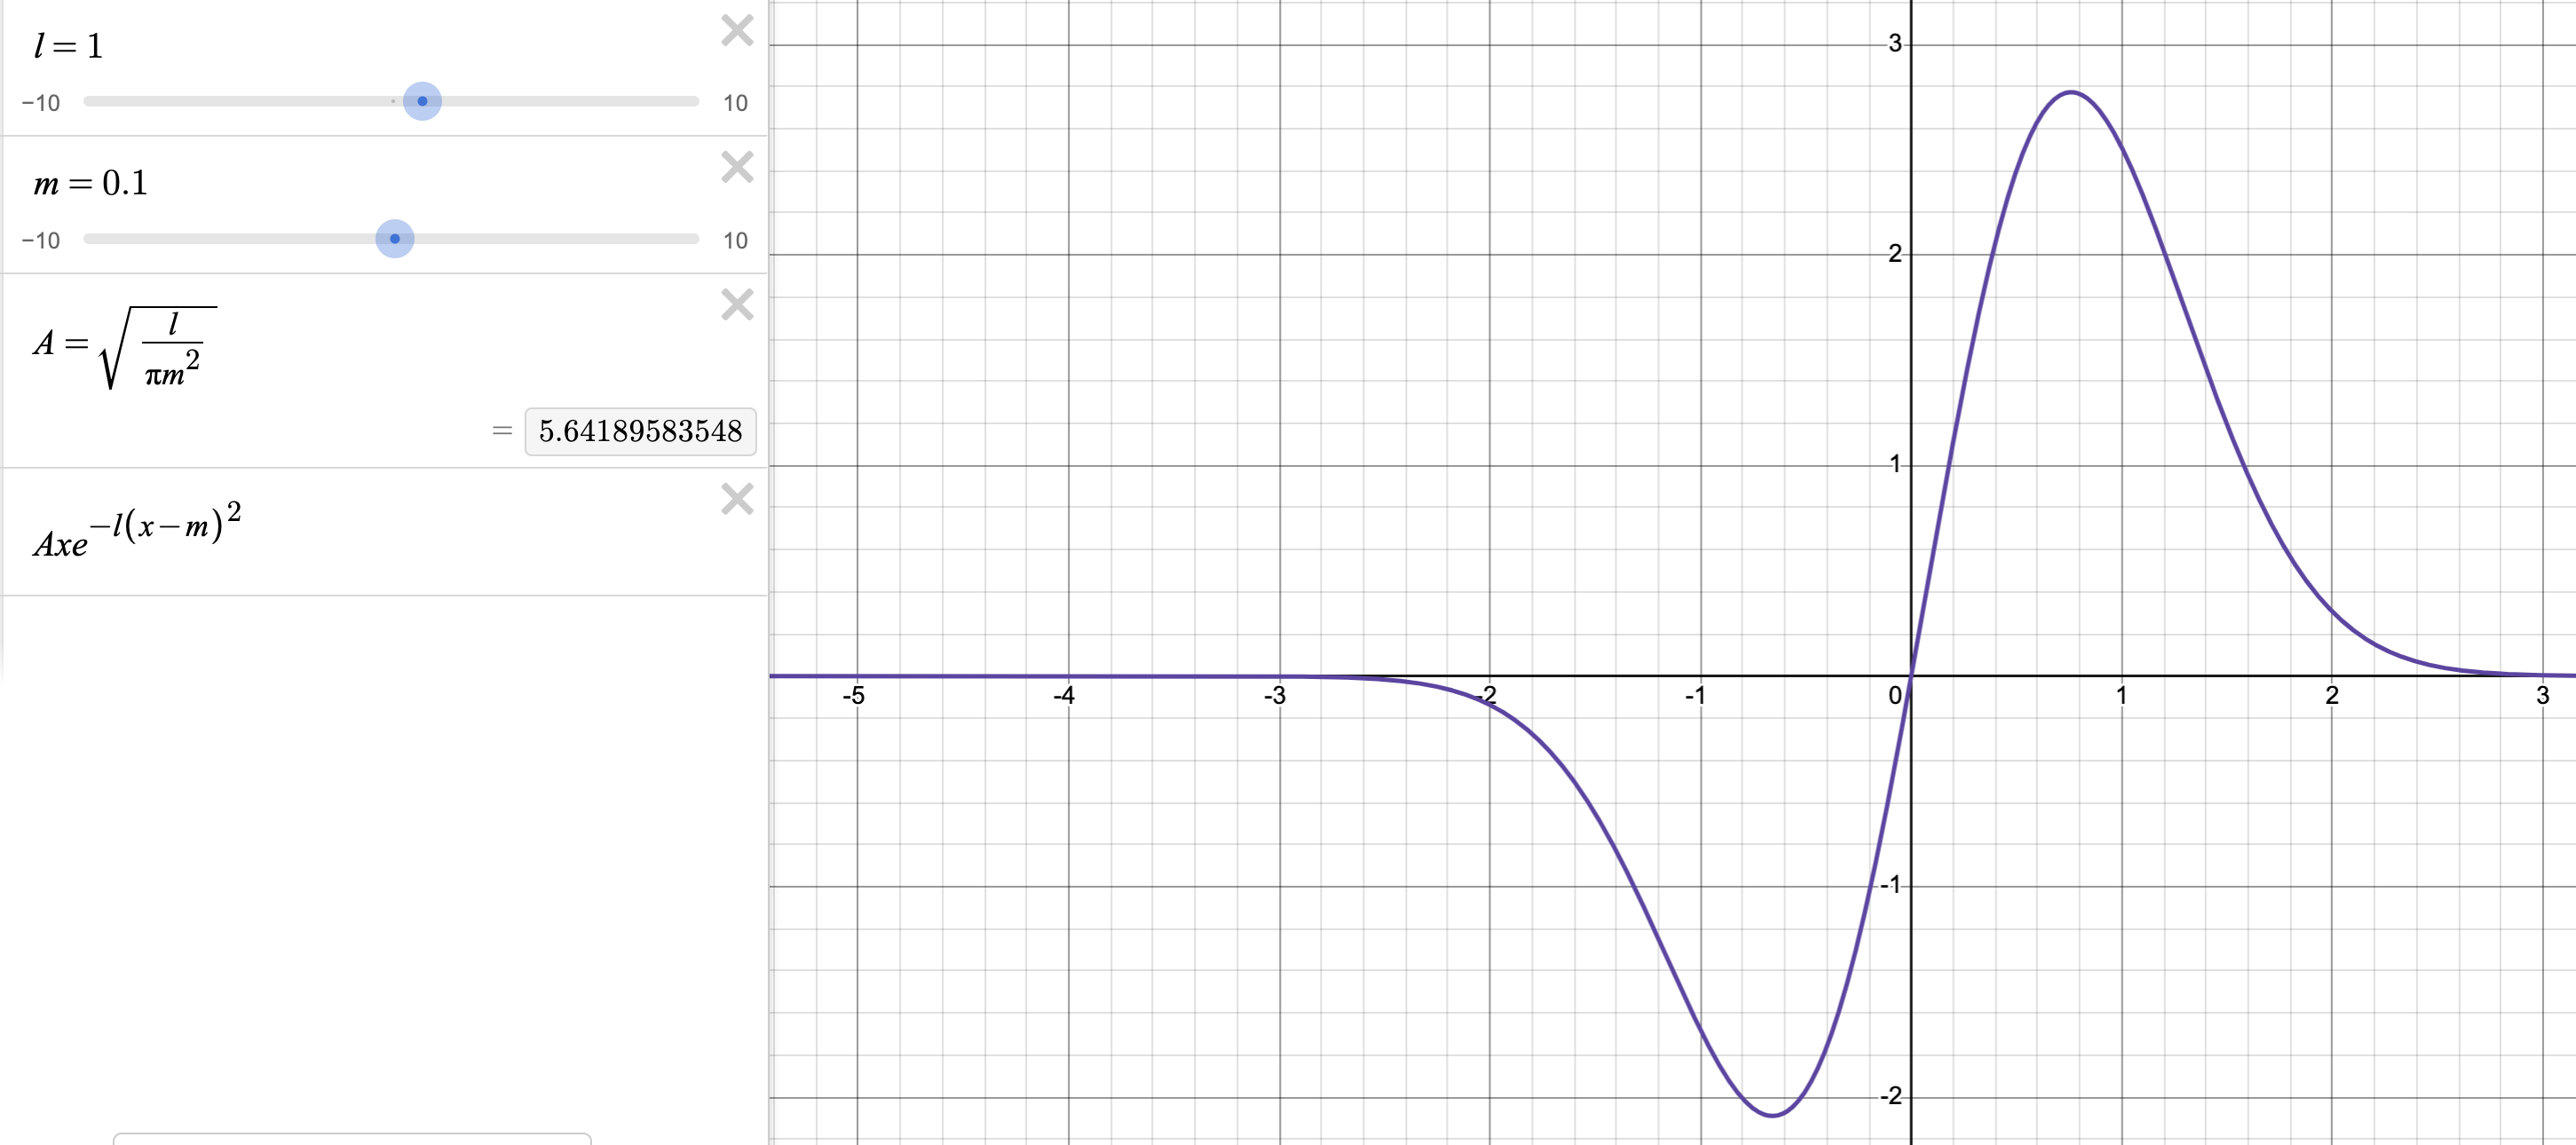
\includegraphics[width=150mm]{q2_b.png}
        \end{figure}

        Overall, even though $\rho(x)$ is normalizable, the reason why $\rho(x)$ is not a probability density function, is because it yields negative values for $x<0$, which is not allowed for general probability density functions.

        \hfil

        \item[(c)] If consider $\rho(x)=Ax^2e^{-\lambda(x-\mu)^2}$, for normalization, consider the following:
        \begin{align}
            \int_{-\infty}^{\infty}\rho(x)dx &= \int_{-\infty}^{\infty}Ax^2e^{-(\sqrt{\lambda}(x-\mu))^2}dx\\&= \frac{1}{\lambda}\int_{-\infty}^{\infty}A(\sqrt{\lambda}(x-\mu))^2e^{-(\sqrt{\lambda}(x-\mu))^2}dx + \int_{-\infty}^{\infty}2\mu x\cdot Ae^{-(\sqrt{\lambda}(x-\mu))^2}dx-\int_{-\infty}^{\infty}A\mu^2e^{-(\sqrt{\lambda}(x-\mu))^2}dx\\
            &= \frac{A}{\lambda\sqrt{\lambda}}\int_{-\infty}^{\infty}u^2e^{-u^2}du + \int_{-\infty}^{\infty}2\mu(\sqrt{\lambda}(x-\mu))\cdot Ae^{-(\sqrt{\lambda}(x-\mu))^2}dx+\int_{-\infty}^{\infty}A\mu^2e^{-(\sqrt{\lambda}(x-\mu))^2}dx\\
            &= \frac{A}{2\lambda}\sqrt{\frac{\pi}{\lambda}}+A\mu^2\sqrt{\frac{\pi}{\lambda}} = A\sqrt{\frac{\pi}{\lambda}}\left(\mu^2+\frac{1}{2\lambda}\right)
        \end{align}
        As a consequence of normalization, $A=\frac{2\lambda}{2\lambda\mu^2+1}\cdot\sqrt{\frac{\lambda}{\pi}}$.

        \hfil

        Now, $\left<x\right>,\left<x^2\right>$ are given as follow:
        \begin{align}
            \left<x\right>&=\int_{-\infty}^{\infty}Ax^3e^{-(\sqrt{\lambda}(x-\mu))^2}dx\\
            &= \frac{1}{\lambda\sqrt{\lambda}}(\sqrt{\lambda}(x-\mu))^3 Ae^{-(\sqrt{\lambda}(x-\mu))^2}dx + \frac{1}{\lambda}\int_{-\infty}^{\infty}3\mu(\sqrt{\lambda}(x-\mu))^2 Ae^{-(\sqrt{\lambda}(x-\mu))^2}dx\\
            &+ \frac{1}{\sqrt{\lambda}}\int_{-\infty}^{\infty}3\mu^2(\sqrt{\lambda}(x-\mu))Ae^{-(\sqrt{\lambda}(x-\mu))^2}dx + \int_{-\infty}^{\infty}\mu^3 Ae^{-(\sqrt{\lambda}(x-\mu))^2}dx\\
            &= \frac{3\mu A}{\lambda\sqrt{\lambda}}\int_{-\infty}^{\infty}u^2e^{-u^2}du + \mu^3 A\sqrt{\frac{\pi}{\lambda}} = \frac{3\mu A}{\lambda}\sqrt{\frac{\pi}{\lambda}}+\mu^3 A\sqrt{\frac{\pi}{\lambda}}\\
            &= \frac{3\mu+\lambda\mu^3}{\lambda}\cdot \frac{2\lambda}{2\lambda\mu^2+1} = \frac{6\mu+2\lambda\mu^3}{2\lambda\mu^2+1}
        \end{align}

        \hfil

        \begin{align}
            \left<x^2\right>&=\int_{-\infty}^{\infty}x^4\cdot Ae^{-(\sqrt{\lambda}(x-\mu))^2}dx\\
            &= \frac{1}{\lambda^2}\int_{-\infty}^{\infty}(\sqrt{\lambda}(x-\mu))^4 Ae^{-(\sqrt{\lambda}(x-\mu))^2}dx+\frac{1}{\lambda\sqrt{\lambda}}\int_{-\infty}^{\infty}4\mu(\sqrt{\lambda}(x-\mu))^3 Ae^{-(\sqrt{\lambda}(x-\mu))^2}dx\\
            &+ \frac{1}{\lambda}\int_{-\infty}^{\infty}6\mu^2(\sqrt{\lambda}(x-\mu))^2 Ae^{-(\sqrt{\lambda}(x-\mu))^2}dx+\frac{1}{\sqrt{\lambda}}\int_{-\infty}^{\infty}4\mu^3(\sqrt{\lambda}(x-\mu))Ae^{-(\sqrt{\lambda}(x-\mu))^2}dx\\
            &+ \int_{-\infty}^{\infty}\mu^4Ae^{-(\sqrt{\lambda}(x-\mu))^2}dx\\
            &= \frac{A}{\lambda^2\sqrt{\lambda}}\int_{-\infty}^{\infty}u^4e^{-u^2}du+\frac{6\mu^2A}{\lambda\sqrt{\lambda}}\int_{-\infty}^{\infty}u^2e^{-u^2}du + \frac{\mu^4A}{\sqrt{\lambda}}\int_{-\infty}^{\infty}e^{-u^2}du\\
            &= \frac{3A}{4\lambda^2}\sqrt{\frac{\pi}{\lambda}} + \frac{3\mu^2A}{\lambda}\sqrt{\frac{\pi}{\lambda}}+\mu^4A\sqrt{\frac{\pi}{\lambda}} = \frac{3+12\mu^2\lambda+4\mu^4\lambda^2}{4\lambda^2}\cdot \frac{2\lambda}{2\lambda\mu^2+1} = \frac{3+12\mu^2\lambda+4\mu^4\lambda^2}{4\lambda^2\mu^2+2\lambda}
        \end{align}
        Hence, the standard deviation $\sigma_x=\sqrt{\left<x^2\right>-\left<x\right>^2}=\sqrt{\frac{3+12\mu^2\lambda+4\mu^4\lambda^2}{4\lambda^2\mu^2+2\lambda}-\left(\frac{6\mu+2\lambda\mu^3}{2\lambda\mu^2+1}\right)^2}$. Which, we have the following sketch:

        \begin{figure}[h!]
            \centering
            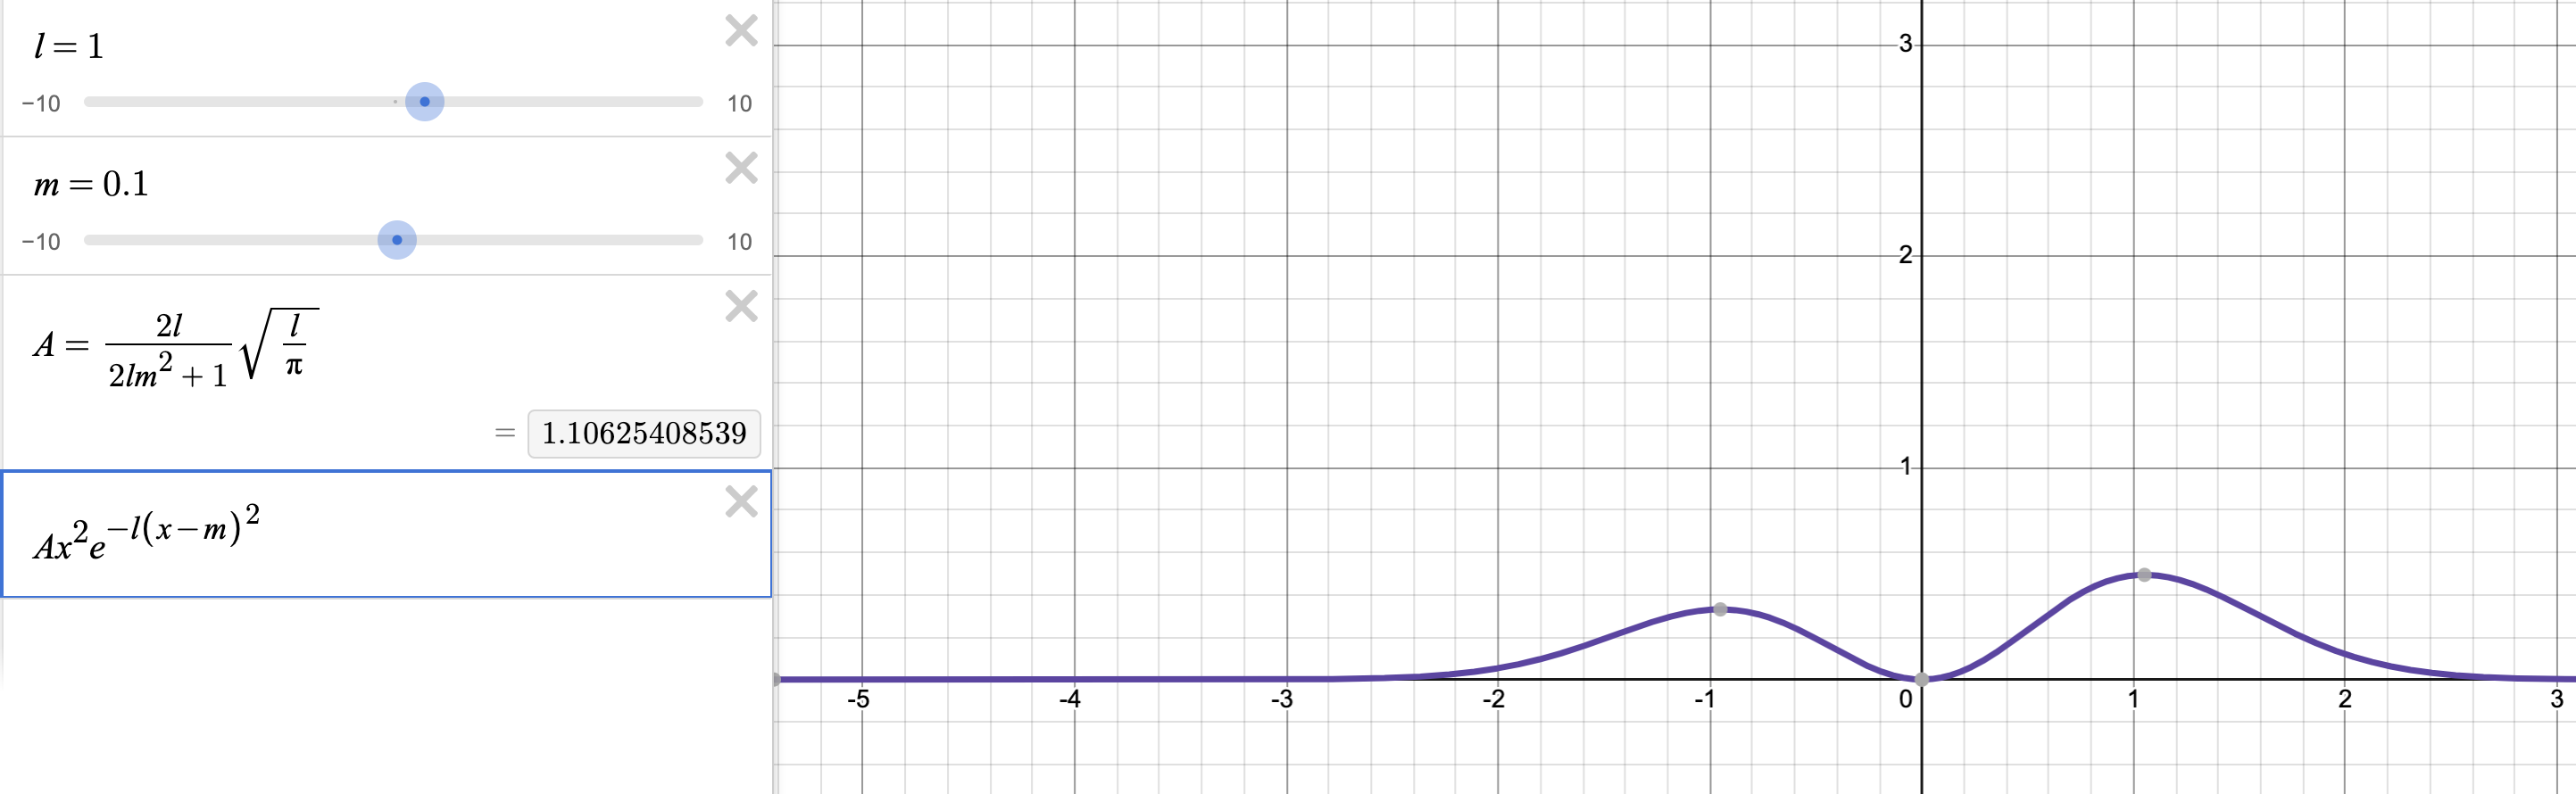
\includegraphics[width=150mm]{q2_c.png}
        \end{figure}

        \hfil

        \item[(d)] Given $\Psi(x)=Ae^{-(x/b)^2}$, for normalization, we get the following integral:
        \begin{align}
            1=\int_{-\infty}^{\infty}|\Psi|^2dx = \int_{-\infty}^{\infty}A^2e^{-(\sqrt{2}x/b)^2}dx = \frac{bA^2}{\sqrt{2}}\int_{-\infty}^{\infty}e^{-u^2}du = A^2\cdot \sqrt{\frac{b^2\pi}{2}}
        \end{align}
        Hence, $A=\left(\frac{2}{b^2\pi}\right)^\frac{1}{4}$.

        \hfil

        Given the normalization, $\left<x\right>$ and $\left<x^2\right>$ are given as:
        \begin{align}
            \left<x\right>&=\int_{-\infty}^{\infty}x|\Psi|^2dx = \int_{-\infty}^{\infty}xA^2e^{-2(x/b)^2}dx = 0
        \end{align}
        (The above is the property of odd functions).

        \begin{align}
            \left<x^2\right>&=\int_{-\infty}^{\infty}x^2|\Psi|^2dx = \frac{b^2}{2}\int_{-\infty}^{\infty}A^2\left(\frac{\sqrt{2}x}{b}\right)^2e^{-(\sqrt{2}x/b)^2}dx\\
            &= \frac{b^3}{2\sqrt{2}}\int_{-\infty}^{\infty}A^2 u^2e^{-u^2}du\\\
            &= \frac{b^3}{2\sqrt{2}}A^2\cdot\left(-\frac{1}{2}\right)u\cdot e^{-u^2}\bigg|_{-\infty}^{\infty}+\frac{b^3}{4\sqrt{2}}A^2\int_{-\infty}^{\infty}e^{-u^2}du\\
            &= \frac{b^3}{4}A^2\cdot\sqrt{\frac{\pi}{2}}=\frac{b^3}{4}\cdot\sqrt{\frac{2}{b^2\pi}}\cdot\sqrt{\frac{\pi}{2}}=\frac{b^2}{4}
        \end{align}
        So, the uncertainty $\sigma_x=\sqrt{\left<x^2\right>-\left<x\right>^2}=\frac{b}{2}$.

        \hfil

        Then, to calclate the uncertainty in momentum, we get:
        \begin{align}
            \left<p\right>=\int_{-\infty}^{\infty}\Psi^*\cdot \frac{\hbar}{i}\frac{\partial}{\partial x}(\Psi) dx = -\frac{2\hbar}{ib^2}\int_{-\infty}^{\infty}A^2e^{-2x^2/b^2}\cdot x dx = 0
        \end{align}
        (Note: the above is again property of odd functions).
        \begin{align}
            \left<p^2\right>&=\int_{-\infty}^{\infty}\Psi^*\cdot(-\hbar^2)\frac{\partial^2}{\partial x^2}(\Psi)dx = \frac{2\hbar^2}{b^2}\int_{-\infty}^{\infty}A^2e^{-2x^2/b^2}dx - \frac{4\hbar^2}{b^4}\int_{-\infty}^{\infty}A^2x^2e^{-2x^2/b^2}dx\\
            &= \frac{2\hbar^2}{b^2}\int_{-\infty}^{\infty}|\Psi|^2dx - \frac{4\hbar^2}{b^4}\left<x^2\right>. = \frac{2\hbar^2}{b^2}-\frac{4\hbar^2}{b^4}\cdot \frac{b^2}{4} = \frac{\hbar^2}{b^2}
        \end{align}
        Hence, the uncertainty $\sigma_p=\sqrt{\left<p^2\right>-\left<p\right>^2} = \frac{\hbar}{b}$.

        Which, $\sigma_x\sigma_p = \frac{b}{2}\cdot\frac{\hbar}{b} = \frac{\hbar}{2}\geq \frac{\hbar}{2}$, so the uncertainty principle holds.
    \end{itemize}
\end{proof}

\newpage

\begin{ques}[Fun with probability densities]\label{q3}
Consider the function
\[
\rho(r) =
\begin{cases}
Ar^2 & r \leq R,\\
0 & r \geq R
\end{cases}
\]
such that $dP = 4\pi \rho(r) r^2 dr$ represents the probability of finding a particle in a spherical shell of thickness $dr$ located at the radial coordinate $r$ in three-dimensional spherical
coordinates.

(a) Determine $A$ by requiring that the probability of finding the particle anywhere is
unity. Don’t forget that we’re in three spatial dimensions.

(b) What is the probability of finding the particle between $r = R/2$ and $r = R$?

(c) Determine $\langle r\rangle$, the average radial position of the particle.
\end{ques}
\begin{proof}

    \hfil

    \begin{itemize}
        \item[(a)] Since $dP=4\pi \rho(r)r^2 dr$ represents the probability of finding a partical in a concentric spherical shell of thickness $dr$ and radius $r$, then the total integral of the probability is given by the following (which runs through all radius $r\geq 0$):
        \begin{align}
            1 = \int_{0}^{\infty}4\pi\rho(r)r^2 dr = \int_{0}^{R}4\pi A r^4dr = \frac{4\pi A}{5}r^5\bigg|_{0}^{R} = \frac{4\pi AR^5}{5}
        \end{align}
        Hence, for normalization to happen, $A = \frac{5}{4\pi R^5}$.
        \item[(b)] For the probability to find the partical in $\frac{R}{2}\leq r\leq R$, we get:
        \begin{align}
            \PP\left(\frac{R}{2}\leq r\leq R\right)=\int_{\frac{R}{2}}^{R}4\pi \rho(r)r^2dr = \frac{4\pi A}{5}r^5\bigg|_{\frac{R}{2}}^{R}=\frac{4\pi }{5}\cdot\frac{5}{4\pi R^5}\left(1-\frac{1}{2^5}\right)R^5 = \frac{31}{32}
        \end{align}
        \item[(c)] To calculate $\left<r\right>$, it's given by the following integral:
        \begin{align}
            \left<r\right>=\int_{0}^{\infty}r \cdot 4\pi \rho(r)r^2 dr = \int_{0}^{R}4\pi A r^5 dr = \frac{4\pi A}{6}r^6\bigg|_{0}^{R} = \frac{2\pi}{3}\cdot \frac{5}{4\pi R^5}R^6=\frac{5R}{6}
        \end{align}
    \end{itemize}
\end{proof}
\newpage

\begin{ques}[Probability currents, Griffiths problem 1.9 and 1.14 modified]\label{q4}
Let $P_{ab}(t)$ be the probability of finding a particle in the range $a < x < b$ at time $t$. Show
that
\[
\frac{dP_{ab}}{dt} = J(a, t) - J(b, t)
\]
where
\[
J(x, t) \equiv \frac{i\hbar}{2m}
\left(
\Psi \frac{\partial\Psi^*}{\partial x}
- \Psi^* \frac{\partial \Psi}{\partial x}
\right).
\]

(a) What are the units of $J(x, t)$? J is called the probability current because it tells you

the rate at which probability is “flowing” past the point $x$. If $P_{ab}(t)$ is increasing,
then more probability is flowing into the region at one end than flows out the other.

(b) Consider a particle described by the wavefunction $\Psi(x, t) = A e^{-amx^2/\hbar} e^{-iat}$. Find $A$
for this wavefunction.

(c) Compute the average velocity $\langle v\rangle = d\langle x\rangle/dt$ for this wavefunction.

(d) Compute the probability current for this wavefunction.
\end{ques}
\begin{proof}
    
    \hfil

    \begin{itemize}
        \item[(a)] Since Probability itself has no unit, then $J$ as a consequence of time derivative of probability, endows with the unit of $1/s$ (where $s$ represents seconds for simplicity).
        \item[(b)] Given $\Psi(x,t)=Ae{-amx^2/\hbar}\cdot e^{-iat}$, then it satisfies the following:
        \begin{align}
            1=\int_{-\infty}^{\infty}|\Psi(x,t)|^2 dx = \int_{-\infty}^{\infty}|A|^2e^{-2amx^2/\hbar}dx = \int_{-\infty}^{\infty}|A|^2e^{-\left(\sqrt{2am/\hbar}x\right)^2}dx
        \end{align}
        Takes substitution $u=\sqrt{2am/\hbar}x$, $du=\sqrt{2am/\hbar}dx$, we get:
        \begin{align}
            1=\frac{|A|^2}{\sqrt{2am/\hbar}}\int_{-\infty}^{\infty}e^{-u^2}du = |A|^2\sqrt{\frac{\pi\hbar}{2am}}
        \end{align}
        Hence, we require $|A|=\left(\frac{\pi\hbar}{2am}\right)^{1/4}$.
        \item[(c)] First, we'll compute the expectation value $\left<x\right>$ (with the same substitution as above):
        \begin{align}
            \left<x\right>=\int_{-\infty}^{\infty}x|\Psi(x,t)|^2dx = |A|^2\int_{-\infty}^{\infty}xe^{-(\sqrt{2am/\hbar}x)^2}dx = 0
        \end{align}
        So, the average velocity $\left<v\right>=\frac{d\left<x\right>}{dt}=0$.
        \item[(d)] Given that $\Psi^*(x,t)=A^*e^{-amx^2/\hbar}\cdot e^{iat}$, $\frac{d\Psi^*}{dx}=-A^*\frac{2amx}{\hbar}e^{-amx^2/\hbar}\cdot e^{iat}$, and $\frac{d\Psi}{dx}=-A\frac{2amx}{\hbar}e^{-amx^2/\hbar}\cdot e^{-iat}$. So, the Probability Current is given by:
        \begin{align}
            J(x,t) &= \frac{i\hbar}{2m}\left(-Ae^{-amx^2/\hbar}e^{-iat}\cdot A^*\frac{2amx}{\hbar}e^{-amx^2/\hbar} e^{iat}+A^*e^{-amx^2/\hbar}e^{iat}\cdot A\frac{2amx}{\hbar}e^{-amx^2/\hbar}e^{-iat}\right)\\
            &=0
        \end{align}
    \end{itemize}
\end{proof}

\newpage

\begin{ques}[More intuition about probability currents]\label{q5}
The wave function of a beam of free particles traveling in one dimension with velocity $v$ is
\[
\Psi(x) = A \exp [ikx]
\]
where $k = mv/\hbar$. (You might notice that this wave function is not strictly normalizable, but
you can set aside this concern for now.) Argue that the probability current corresponding
to this beam of particles has the form
\[
J(x) = v \times \text{density of particles}.
\]
\end{ques}

\begin{proof}
    Given the definition of probability current $J(x,t):=-\frac{i\hbar}{2m}\left(\Psi^*\frac{\partial \Psi}{\partial x}-\frac{\partial \Psi^*}{\partial x}\Psi\right)$, with $\Psi(x,t)=Ae^{ikx}$, then we have $\frac{\partial \Psi}{\partial x}=Aike^{ikx}$ and $\frac{\partial \Psi^*}{\partial x}=-Aike^{-ikx}$. Hence, $J$ expands to the following form:
    \begin{align}
        J(x,t)=-\frac{i\hbar}{2m}\left(Ae^{-ikx}\cdot Aike^{ikx}+Aike^{-ikx}\cdot Ae^{ikx}\right) = \frac{\hbar}{m}\cdot A^2k=A^2\frac{\hbar}{m}\cdot \frac{mv}{\hbar} = vA^2
    \end{align}
    Now, given that $\int_{a}^{b}|\Psi|^2dx$ is the probability of finding particles in the range of $[a,b]$ (assume $a<b$), we yield the following (recall that $|e^{ikx}|=1$):
    \begin{align}
        \int_{a}^{b}|\Psi|^2 dx=\int_{a}^{b}A^2 dx = A^2\cdot (b-a)
    \end{align}
    Which, classically given a beam of a particle, the probability of finding a particle in the range of $[a,b]$ can be thought of as the density $\lambda \cdot (b-a)$ (which denotes the amount of particles within a certain range). Hence, here if $A^2\cdot (b-a)$ serves the purpose for arbitrary interval $[a,b]$ (with $a<b$), then $A^2$ must serve as the density of the bea of free particles.

    Hence, $J = vA^2$ is in terms of $v \times $ density of the particles.

\end{proof}

\hfil

\begin{ques}[Classical Particle in a Well (Griffiths Problem 1.11)]\label{q6}
Imagine a particle of mass $m$ and energy $E$ in a potential well $V (x)$, sliding frictionlessly
back and forth between the classical turning points (call them $a$ and $b$). Classically, the
probability of finding the particle in the range $dx$ (if, for example, you took a snapshot at
a random time $t$) is equal to the fraction of the time $T$ it takes to get from $a$ to $b$ that it
spends in the interval $dx$:
\[
\rho(x)dx = \frac{dt}{T} = \frac{(dt/dx)dx}{T} = \frac{1}{v(x)T} dx
\]
where $v(x)$ is the speed, and
\[
T = \int_0^T dt = \int_a^b \frac{1}{v(x)} dx .
\]
Thus
\[
\rho(x) = \frac{1}{v(x)T}.
\]

(a) Use conservation of energy to express $v(x)$ in terms of $E$ and $V(x)$.

(b) As an example, find $\rho(x)$ for the simple harmonic oscillator, $V(x) = kx^2/2$. Plot $\rho(x)$
and check that it is correctly normalized.

(c) For the classical harmonic oscillator in part (b), find $\langle x\rangle$, $\langle x^2\rangle$, and $\sigma_x$.
\end{ques}

\begin{proof}
    \hfill

    \begin{itemize}
        \item[(a)] Assume the conservation of energy, the particle has mass $m$, total energy $E$, and the potential is recorded by $V(x)$. Then, the kinetic energy of the particle is $K=\frac{1}{2}mv(x)^2=E-V(x)$, hence $v(x)=\sqrt{\frac{2(E-V(x))}{m}}$.
        \item[(b)] Given $V(x)=\frac{kx^2}{2}$,  then based on formula in part (a), $v(x)=\sqrt{\frac{2E-kx^2}{m}}$, hence the time $T$ is:
        \begin{align}
            T&=\int_{a}^{b}\frac{1}{v(x)}dx = \int_{a}^{b}\frac{\sqrt{m}}{\sqrt{2E}\cdot \sqrt{1-\left(\sqrt{\frac{k}{2E}}x\right)^2}}dx = \sqrt{\frac{m}{2E}}\cdot\sqrt{\frac{2E}{k}}\int_{\sqrt{\frac{k}{2E}}a}^{\sqrt{\frac{k}{2E}}b}\frac{1}{\sqrt{1-u^2}}du\\
            &= \sqrt{\frac{m}{k}}\arcsin(u)\bigg|_{\sqrt{\frac{k}{2E}}a}^{\sqrt{\frac{k}{2E}}b}
        \end{align}
        Given that $V(x)=kx^2/2$, then the turning point (if assume $a<b$) satisfies $a=-b$ (since the turning points must have the same potential, so $ka^2/2=kb^2/2$, or $a=\pm b$; with $a<b$, we have $a=-b$, if assuming $b>0$). Hence, the above equation provides $T=2\sqrt{\frac{m}{k}}\arcsin\left(\sqrt{\frac{k}{2E}}b\right)$.

        Using this information, we have: 
        \begin{align}
            \rho(x)=\frac{1}{v(x)T} = \frac{1}{2\sqrt{m/k}\arcsin\left(\sqrt{\frac{k}{2E}}b\right)}\cdot\sqrt{\frac{m}{2E-kx^2}} = \frac{1}{2\arcsin\left(\sqrt{\frac{k}{2E}}b\right)}\cdot\sqrt{\frac{k}{2E-kx^2}}
        \end{align}
        Also, given that at $x=b$, $V(b)=E$ (the criterion for turning point), then $kb^2/2=E$, or $b=\sqrt{\frac{2E}{k}}$. Which, $\rho(x)$ simplifies to:
        \begin{align}
            \rho(x)=\frac{1}{2\arcsin(1)}\sqrt{\frac{k}{2E-kx^2}}=\frac{1}{\pi}\sqrt{\frac{k}{2E-kx^2}}
        \end{align}
        To check that $\rho(x)$ is normalized, consider its integral on $(-b,b)$ (the open interval between the two turning points), based on assumption one has $V(x)=kx^2/2< E$ for all $x \in (-b,b)$, hence  $2E-kx^2> 0$ on this interval. Perform the integral, one gets:
        \begin{align}
            \int_{-b}^{b}\rho(x)dx &= \frac{1}{2\arcsin\left(\sqrt{\frac{k}{2E}}b\right)}\int_{-b}^{b}\sqrt{\frac{k}{2E-kx^2}}dx=\frac{1}{2\arcsin\left(\sqrt{\frac{k}{2E}}b\right)}\int_{-b}^{b}\frac{\sqrt{k}}{\sqrt{2E}\cdot\sqrt{1-\left(\sqrt{\frac{k}{2E}}x\right)^2}}dx\\
            &= \frac{1}{2\arcsin\left(\sqrt{\frac{k}{2E}}b\right)}\cdot\sqrt{\frac{k}{2E}}\cdot \sqrt{\frac{2E}{k}}\int_{-\sqrt{\frac{k}{2E}}b}^{\sqrt{\frac{k}{2E}}b}\frac{1}{\sqrt{1-u^2}}du = \frac{1}{2\arcsin\left(\sqrt{\frac{k}{2E}}b\right)}\cdot\arcsin(u)\bigg|_{-\sqrt{\frac{k}{2E}}b}^{\sqrt{\frac{k}{2E}}b}\\
            &= \frac{1}{2\arcsin\left(\sqrt{\frac{k}{2E}}b\right)}\cdot 2\arcsin\left(\sqrt{\frac{k}{2E}}b\right)=1
        \end{align}
        Hence, $\rho(x)$ is perfectly normalized.

        Finally, here is a graph of $\rho(x)$, with the constant given on the side:
        \begin{figure}[h!]
            \centering
            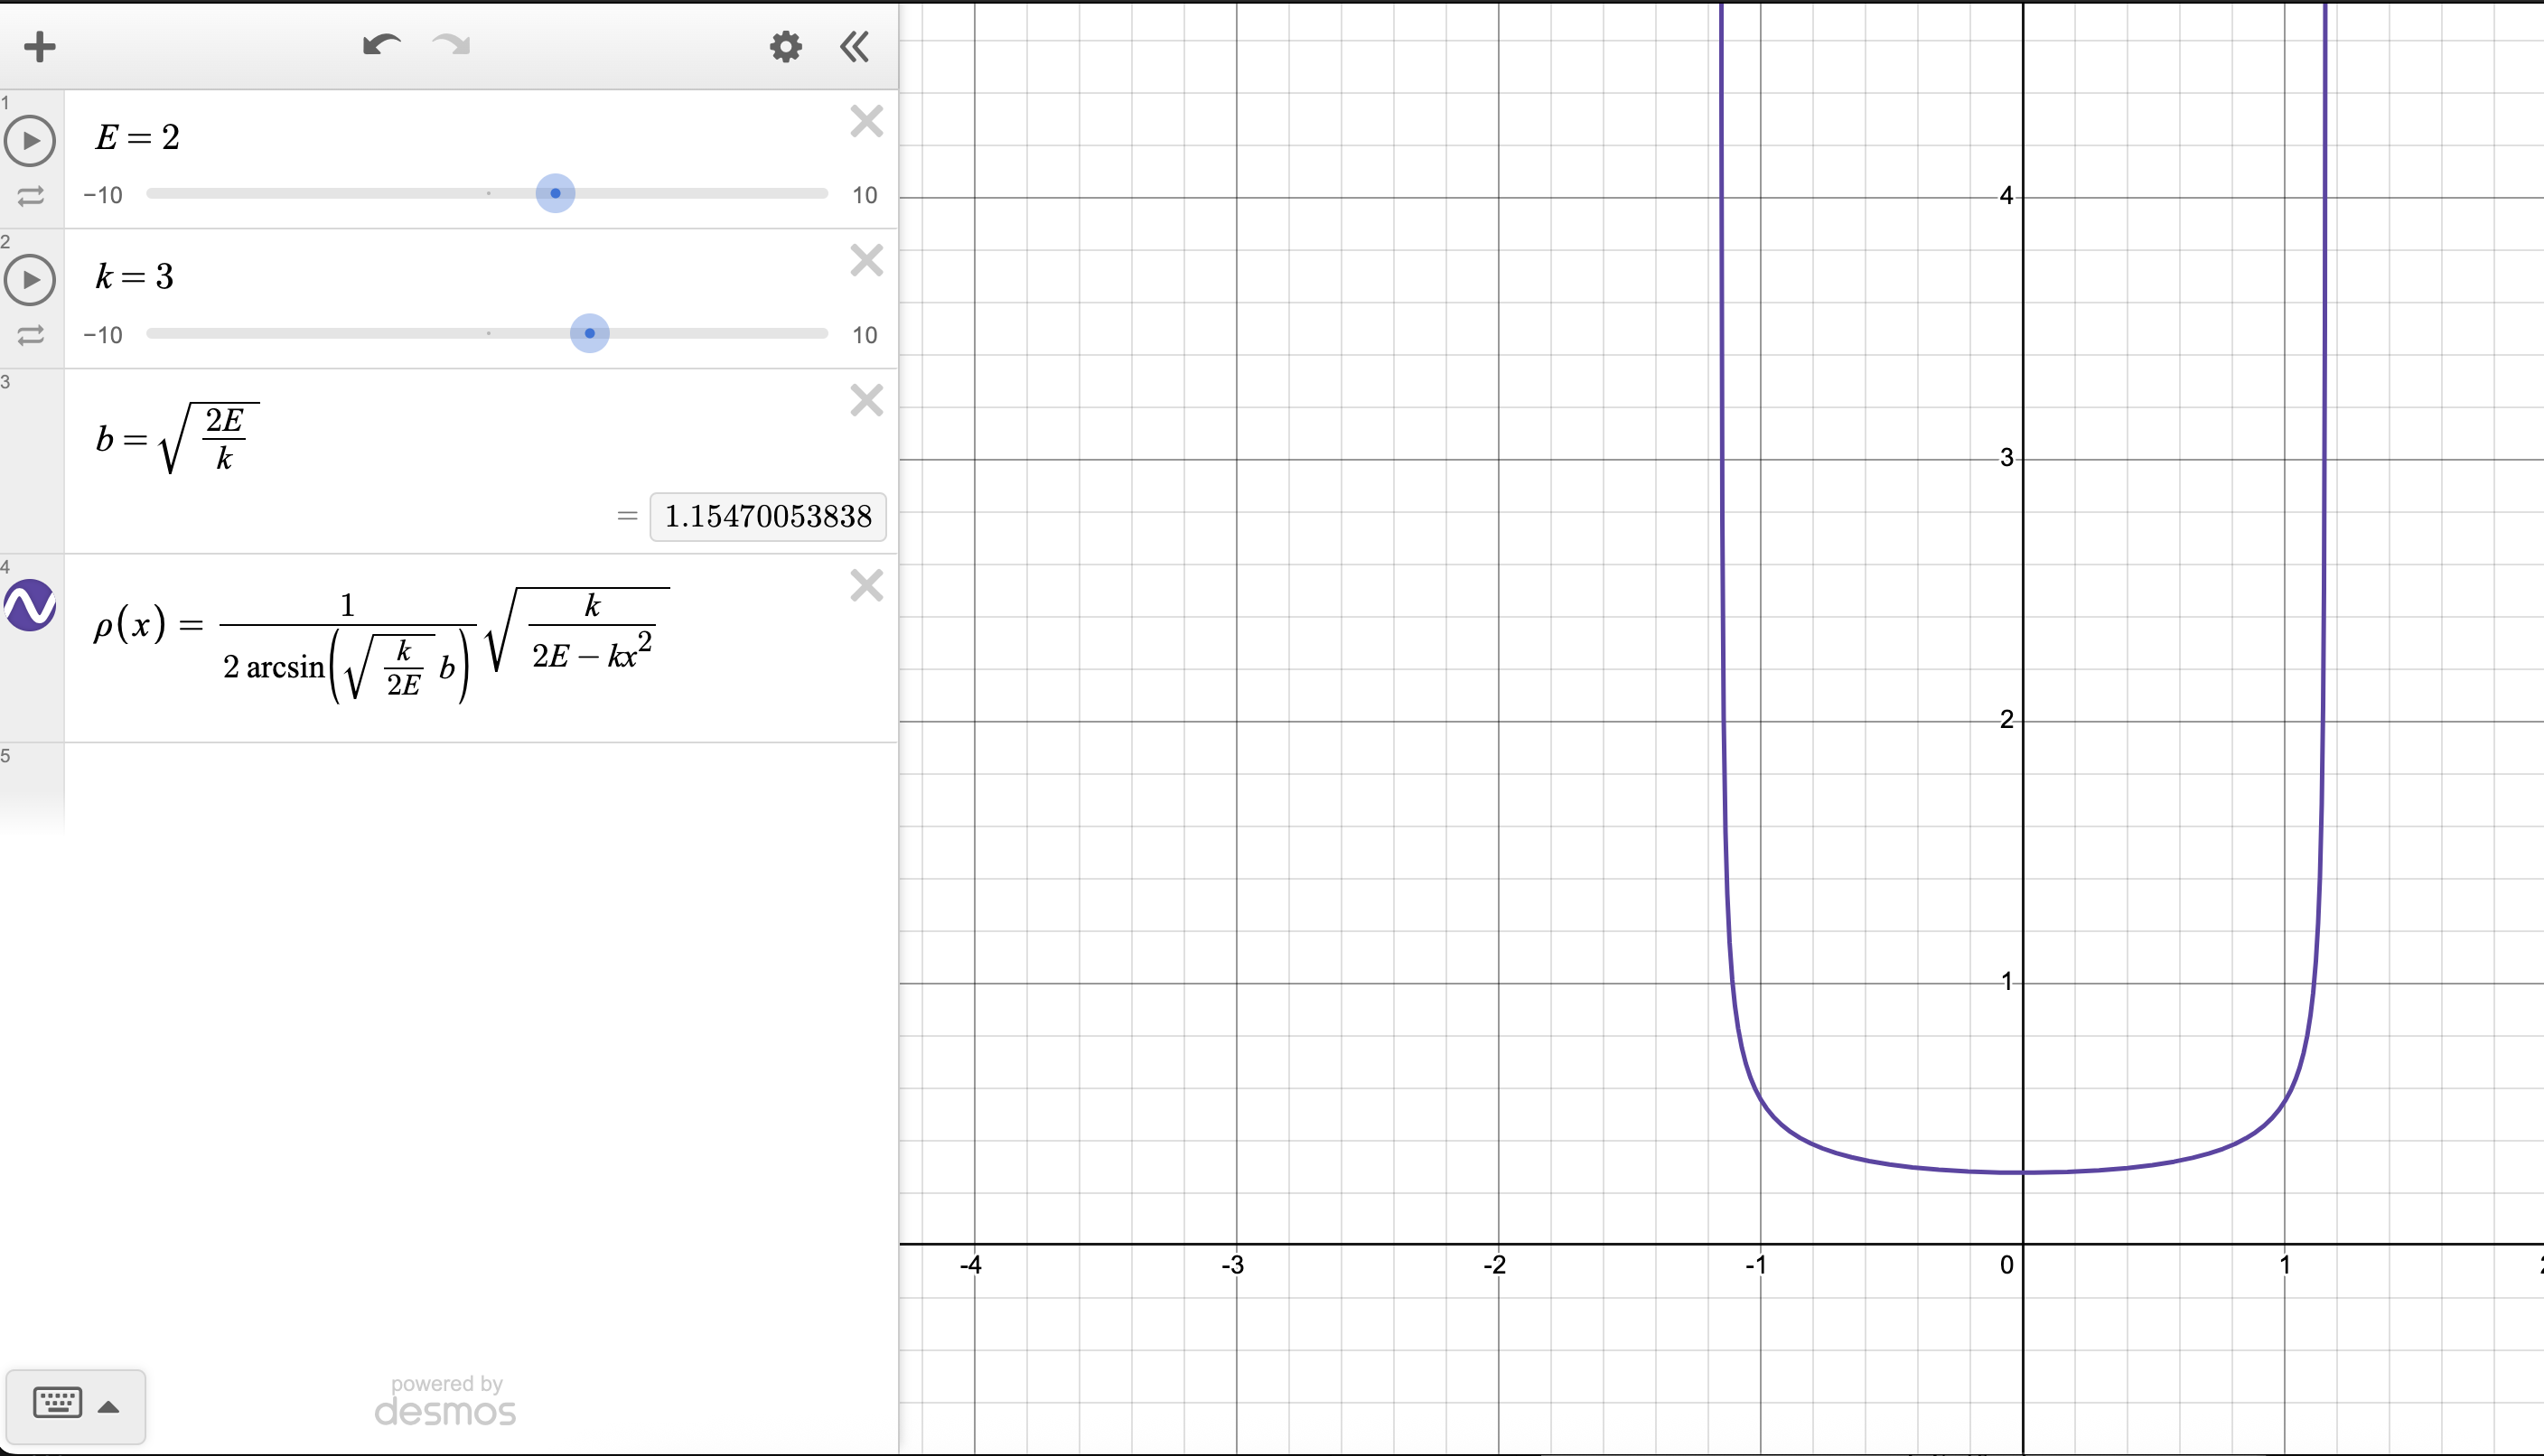
\includegraphics[width=150mm]{q6_graph.png}
        \end{figure}
        \item[(c)] To find $\left<x\right>,\left<x^2\right>$, consider the following integrals:
        \begin{align}
            \left<x\right>&= \int_{-b}^{b}x\rho(x)dx = \int_{-b}^{b}x\sqrt{\frac{k}{2E-kx^2}}dx = 0
        \end{align}
        (The above integral is $0$ since eventually it's an integral of odd function with integration bounds of opposite signs).

        \begin{align}
            \left<x^2\right>&=\int_{-b}^{b}x^2\rho(x)dx = -\frac{1}{2k}\int_{-b}^{b}x\cdot (-2kx)\sqrt{\frac{k}{2E-kx^2}}dx\\
            &= -\frac{1}{2k}x\cdot2\sqrt{k}\cdot \sqrt{2E-kx^2}\bigg|_{-b}^{b} + \frac{1}{2k}\int_{-b}^{b}2\sqrt{k}\cdot\sqrt{2E-kx^2}dx\\
            &= -\frac{2}{\sqrt{k}}b\cdot \sqrt{2E-kb^2} + \sqrt{\frac{2E}{k}}\int_{-b}^{b}\sqrt{1-\left(\sqrt{\frac{k}{2E}}x\right)^2}dx\\
            &= -\frac{2b}{\sqrt{k}}\sqrt{2E - k\cdot \left(\sqrt{\frac{2E}{k}}\right)^2}+\frac{2E}{k}\int_{-\sqrt{\frac{k}{2E}}b}^{\sqrt{\frac{k}{2E}}b}\sqrt{1-u^2}du\\
            &= 0+\frac{2E}{k}\int_{-1}^{1}\sqrt{1-u^2}du = \frac{2E}{k}\cdot\frac{\pi}{2}=\frac{E\pi}{k}
        \end{align}
        With this value, then the final one $\sigma_x=\sqrt{\left<x^2\right>-\left<x\right>^2} = \sqrt{\frac{E\pi}{k}}$.
    \end{itemize}
\end{proof}

\newpage

\begin{ques}[Unstable Particles (Griffiths Problem 1.17)]\label{q7}
Suppose you wanted to describe an unstable particle, that spontaneously disintegrates with
a “lifetime” $\tau$. In that case, the total probability of finding the particle somewhere should
not be constant, but should decrease at (say) an exponential rate:
\[
P (t) = \int_{-\infty}^{\infty} |\Psi(x, t)|^2 dx = e^{-t/\tau}.
\]

A crude way of achieving this result is as follows. In Griffiths Eq. 1.24 we tacitly assumed
that $V$ (the potential energy) is real. That is certainly reasonable, but it leads to the
“conservation of probability” enshrined in Griffiths Eq. 1.27. What if we assign to $V$ an
imaginary part,
\[
V = V_0 - i\Gamma
\]
where $V_0$ is the true (real) potential energy and $\Gamma$ is a positive real constant?

(a) Show that (in place of Griffiths Eq. 1.27, i.e.
$\tfrac{d}{dt}\int_{-\infty}^\infty |\Psi(x, t)|^2dx = 0$) we now get
\[
\frac{dP}{dt} = -\frac{2\Gamma}{\hbar}P.
\]

(b) Solve for $P(t)$, and find the lifetime of the particle in terms of $\Gamma$.
\end{ques}

\begin{proof}

    \hfil

    \begin{itemize}
        \item[(a)] Given that $|\Psi(x,t)|^2=\Psi(x,t)\cdot \Psi^*(x,t)$, and $\frac{d}{dt}\int_{-\infty}^{\infty}|\Psi(x,t)|^2dx = \int_{-\infty}^{\infty}\frac{\partial}{\partial t}|\Psi(x,t)|^2 dx$ (i.e. Leibniz Rule applies), together with the Schrodinger's Equation $i\hbar \frac{\partial \Psi}{\partial t}=-\frac{\hbar^2}{2m}\frac{\partial^2\Psi}{\partial x^2}+V\Psi$, we get the following:
        \begin{align}
            \frac{\partial}{\partial t}\left(|\Psi(x,t)|^2\right) &= \frac{\partial }{\partial t}\left(\Psi \Psi^*\right) = \Psi^*\frac{\partial\Psi}{\partial t}+\Psi\frac{\partial \Psi^*}{\partial t}\\
            &= \Psi^*\left(\frac{i\hbar}{2m}\frac{\partial^2\Psi}{\partial x^2}-\frac{i}{\hbar}V\Psi\right)+ \Psi\left(-\frac{i\hbar}{2m}\frac{\partial^2\Psi}{\partial x^2}+\frac{i}{\hbar}V^*\Psi^*\right)\\
            &=\frac{i\hbar}{2m}\left(\Psi^*\frac{\partial^2\Psi}{\partial x^2}-\Psi\frac{\partial^2\Psi^*}{\partial x^2}\right)-\frac{i}{\hbar}\left((V_0-i\Gamma)-(V_0+i\Gamma)\right)|\Psi|^2\\
            &= \frac{i\hbar}{2m}\frac{\partial}{\partial x}\left(\Psi^*\frac{\partial\Psi}{\partial x}-\Psi\frac{\partial\Psi^*}{\partial x}\right)- \frac{2\Gamma}{\hbar}|\Psi|^2
        \end{align}
        Perform integration, we get:
        \begin{align}
            \frac{dP}{dt}&=\frac{d}{dt}\int_{-\infty}^{\infty}|\Psi|^2dx = \int_{-\infty}^{\infty}\frac{\partial}{\partial t}|\Psi|^2 dx = \int_{-\infty}^{\infty}\frac{i\hbar}{2m}\left(\Psi^*\frac{\partial\Psi}{\partial x}-\Psi\frac{\partial\Psi^*}{\partial x}\right)dx- \frac{2\Gamma}{\hbar}\int_{-\infty}^{\infty}|\Psi|^2dx\\
            &= -\frac{2\Gamma}{\hbar}P
        \end{align}
        The first integral is $0$ because of the boundary condition of probability current, while the second integral (up to some constant) yields $P$.
        \item[(b)] To solve for $P(t)$, since $\frac{dP}{dt}=-\frac{2\Gamma}{\hbar}P$, we get $P(t)=Ke^{-2\Gamma t/\hbar}$ for some undetermined coefficient $K$. Which, if the lifetime $\tau$ of the particle is given as $P(t)=Ke^{-t/\tau}$, then here $\tau=\frac{\hbar}{2\Gamma}$.
    \end{itemize}
\end{proof}

\end{document}